\chapter{Simulation Study} \label{chap:simulation}

\section{Conditions} \label{sec:conditions}

A simulation study was conducted to assess three attributes of the bayesian implementation of the GLLAMM for dichotomous outcomes:
%
\begin{enumerate}
	%
	\item \textbf{Performance.} The study assessed the performance of the MCMC chains, in terms of achieving stationarity, convergence and good mixing,  under centered (CP) and non-centered parametrization (NCP), respectively.
	%
	\item \textbf{Recovery capacity.} The study evaluated the capacity to recover the parameters of interest, e.g. regression parameters, latent variables and loadings. However, it centered its focus on the recovery of the regression parameters, as they are highly relevant for making appropriate inferences at the individual level.
	%
	\item \textbf{Retrodictive accuracy.} The study appraised the capacity of the implementation to retrodict the data of interest, according to a set of aggregation dimensions.
	%
\end{enumerate} 

\noindent In this context, a fully crossed design with $3 \times 2 \times 2$ experimental conditions was proposed. 

First, the author used three different samples sizes to generate the data under analysis: $500$, $250$, and $100$. The literature on IRT models present several implementations with samples sizes above $250$, however, few present samples lower than that. The author decided to use a sample size of a $100$ to fill in this gap. Moreover, the decision was also supported by the notion that the change of the posterior sampling geometries could benefit the performance, and recovery capacity of the implementation, under this setting.

Second, as expected, the author used two parametrization of the models: CP and NCP. To the author's knowledge, the IRT literature has not evaluated the change of posterior sampling geometries, as an alternative to improve the performance of the bayesian implementation of said models. This study is set to fill in part of this gap.

Third, the author evaluated the performance, recovery capacity and retrodictive accuracy of a first-order and second-order latent variable models (FOLV and SOLV, respectively). The decision was based on the literature of Confirmatory Factor Analysis (CFA), where before fitting a SOLV model (figure \ref{fig:SOLV_model}), the researcher need to asses if the correlation structure at the first level of the FOLV model (figure \ref{fig:FOLV_model}) justifies the decision.

Therefore, ten ($10$) data sets were generated for each study condition, following the algorithm in section \ref{sect:algorithm}. Each data set resembled responses to $25$ binary scored items, conforming to the SOLV model defined in figure \ref{fig:SOLV_model}. The model was motivated by the hypothesized structure for the reading comprehension sub-test, from the Peruvian public teaching career national assessment (see chapter \ref{chap:application}). The latent structure, regression parameters, and loadings remained unchanged throughout the simulation replicas, to reduce experimental error \cite{Kieftenbeld_et_al_2012}. 

%%%%%%%%%%%%%%%%%%%%%%%%%%%%%%%%%%%%%%%%%%%%%%%%%%%%%%%%%%%%%%%%%%%%%%%

\section{Algorithm} \label{sect:algorithm}

Each data replication was simulated following a six-step procedure. First, the author randomly simulated a collection of pseudo-covariates $\mathbf{W}_{\theta} = [ W_{1}, W_{2}, W_{3}, W_{4} ]$, motivated by a similar information set present in the reading comprehension sub-test. The generated covariates were: (i) a binary ``gender" variable ($W_{1}$), describing males and females, (ii) an integer ``age" variable ($W_{2}$) with range $[30, 65]$, the latter corresponding to the age of retirement, (iii) a three-level categorical ``education" variable ($W_{3}$), indicating the type of education the individual received: institute only, university only, or both; and finally (iv) a four-level categorical ``experience" variable ($W_{4}$), denoting the individual's years of work experience, where the higher the category, the higher the years of experience. Associated with these, the author defined their regression parameters $\mathbf{\Gamma}_{\theta} = [\Gamma_{0}, \Gamma_{1}, \Gamma_{2}, \Gamma_{3}, \Gamma_{4}]$ where: (i) $\Gamma_{0} = 0$, indicating the absence of an intercept; (ii) $\Gamma_{1} = [\gamma_{m}, \gamma_{f}] = [0, 1]$, for males and females, respectively; (iii) $\Gamma_{2} = -0.01$, indicating the individuals loose ability with age, in a linear manner; (iv) $\Gamma_{3} = [\gamma_{io}, \gamma_{uo}, \gamma_{b}] = [-0.5, 0.5, 0]$, assuming individuals with university degree have better ability levels, followed by individuals with both educations, and last individuals with institute degrees; and lastly (v) $\Gamma_{4} = [\gamma_{0y}, \gamma_{5y}, \gamma_{10y}, \gamma_{11+y}] = [-0.5, 0, 0.35, 0.5]$, implying experience has decreasing returns on abilities.

Second, the study simulated the second- and first-order latent variables, corresponding to the reading comprehension ability and its three sub-dimensions: literal, inferential and reflective. Reading comprehension ($\theta^{(3)}_{j}$) was generated from a normal distribution $N( \mu^{(3)}_{j}, \sigma^{(3)}_{\theta} )$, with $\mu^{(3)}_{j} = \pmb{\Gamma}_{\theta} \; \mathbf{W}_{\theta}$, i.e. the linear combination of the simulated covariates and its corresponding regression parameters, and $\sigma^{(3)}_{\theta}=0.5$. On the other hand, the three sub-dimensions were generated from a multivariate normal distribution $MVN( \mu^{(2)}_{j.} , \Sigma^{(2)})$, with $\mu^{(2)}_{j.} = [\mu^{(2)}_{j1}, \mu^{(2)}_{j2}, \mu^{(2)}_{j3}] = [\lambda^{(2)}_{1} \theta^{(3)}_{j}, \; \lambda^{(2)}_{2} \theta^{(3)}_{j}, \; \lambda^{(2)}_{3} \theta^{(3)}_{j} ]$, and $\Sigma^{(2)} = S^{(2)} R^{(2)} S^{(2)}$. In order to ensure the FOLV model in figure \ref{fig:FOLV_model} lead us to the SOLV in figure \ref{fig:SOLV_model}, the author assumed loadings $\pmb{\lambda}^{(2)} = [\lambda^{(2)}_{1}, \lambda^{(2)}_{2}, \lambda^{(2)}_{3}] = [0.95, 0.95, 0.95]$. Using Wright's tracing rules \cite{Beaujean_2014}, the latter implies the sub-dimension would have an approximate unconditional correlation of $0.95 \times 0.94 = 0.9025$. Lastly, $S^{(2)} = \sigma^{(2)}_{\theta} I$, i.e. a diagonal standard deviation matrix with $\sigma^{(2)}_{\theta} = 0.5$; whereas $R^{(2)} = I$, i.e. an identity correlation matrix, implying the sub-dimensions are independent after accounting reading comprehension.

Third, the author defined five ($5$) common stimulus or texts for the items, where the mean difficulty for the texts $\pmb{\eta}^{(3)} = [\eta^{(3)}_{1}, \eta^{(3)}_{2}, \eta^{(3)}_{3}, \eta^{(3)}_{4}, \eta^{(3)}_{5}] = [-1.50, -0.75, 0, 0.75, 1.50]$; whereas the deviation from said mean difficulties were $\sigma^{(3)}_{\eta} = 0.5$ for all texts. 

Fourth, $25$ items were randomly generated from independent normal distributions $N( \mu^{(2)}_{k}, \sigma^{(2)}_{k} ) $, with $\mu^{(2)}_{k} = \pmb{\eta}^{(3)} \pmb{\alpha}^{(2)} \mathbf{A}$ and $\sigma^{(2)}_{k} = \sigma^{(3)}_{k}$; where $\pmb{\alpha}^{(2)} = \mathbf{1}$, indicating the difficulty of the common stimulus directly explained the difficulty of the items, and $\mathbf{A}$ was a block design matrix that maps the items to its corresponding passage, defined in the previous step. Lastly, the dimensions the items were designed to measure were also generated at random.

Fifth, the author calculated the linear predictor $v_{jkd}$ and probability of endorsing an item $\pi_{jkd}$, for each individual $j$ on item $k$ (belonging to dimension $d$), according to equations (\ref{eq:linear_predictor2}), (\ref{eq:systematic}), and (\ref{eq:response_dich1}), respectively; where the probability was calculated using the logistic inverse-link function.
	
Sixth and last, the outcome $y_{jkd}$ was simulated from a Bernoulli distribution as in equation (\ref{eq:distributional}), with a probability of success calculated as in the previous step.

The code associated with the full simulation process can be found in Appendix \ref{appC2_1:sim}.

%%%%%%%%%%%%%%%%%%%%%%%%%%%%%%%%%%%%%%%%%%%%%%%%%%%%%%%%%%%%%%%%%%%%%%%
%%%%%%%%%%%%%%%%%%%%%%%%%%%%%%%%%%%%%%%%%%%%%%%%%%%%%%%%%%%%%%%%%%%%%%%

\section{Parameter estimation}

\subsection{Models and identification}

As stated in previous sections, we analyze two models: (i) a FOLV model depicted in figure \ref{fig:FOLV_model}, and (ii) a SOLV model depicted in figure \ref{fig:SOLV_model}.

In order to fully specify the model and provide a scale for the latent variables, the current research decided set the scale of the higher order dimension and sub-dimensions to one, i.e. $\sigma^{3}_{\theta} = 1$, and $S^{(2)} = \sigma^{(2)}_{\theta} I$ with $\sigma^{(2)}_{\theta} = 1$, commonly know as the unit variance identification scheme (UVI). 

Notice we need to set the scales for all the dimensions, because otherwise the latent structure would not be identified. At the level of the FOLV (level-2), we would have $(3 \times 4)/2 = 6$ pieces of information available to estimate $10$ parameters, i.e. $3$ loadings, $4$ variances corresponding to the FOLV and SOLV, and $3$ correlations among sub-dimensions. Therefore, by restricting the variances to one, we have enough information to estimate the other parameters of interest (loadings and correlations). Additionally, this is further justified by the fact that latent variables have no inherent unit in which they are measured, consequently, setting their scale is an arbitrary  decision \cite{Beaujean_2014}.


%%%%%%%%%%%%%%%%%%%%%%%%%%%%%%%%%%%%%%%%%%%%%%%%%%%%%%%%%%%%%%%%%%%%%%%

\subsection{Prior elicitation}

As it was outlined in section \ref{sub_sect:prior_pred}, we will use prior predictive investigation to assess and visualize the consequences of our prior assumptions. The implications will be assessed from two perspectives: the IRT and the outcome space perspective. For the former, we will investigate what the whole set of priors imply for the item characteristic curves (ICC), and item information function (IIF). For the latter, we will examine how the prior assumption translate onto the outcome space.

First, it will useful to define the ICC and IIF functions. \citet{Hambleton_et_al_1991b} defined the ICC as the mathematical function that relates the probability of success on an item, to the ability measured by that same item. In our current implementation, such function would be the systematic part of the GLLAMM, as defined in equations (\ref{eq:systematic}) and (\ref{eq:response_dich1}):
%
\begin{equation} \label{eq:ICC}
	\begin{split}
		\text{ICC} \left( \theta^{(l)}_{jd} \right) & = \pi_{jkd} = \frac{ \text{exp}(v_{jkd}) }{ 1 + \text{exp}(v_{jkd}) }
	\end{split}	
\end{equation}

\noindent where the linear predictor $v_{jkd}$ contains the item difficulty $\eta^{(2)}_{k}$ and the individual's ability $\theta^{(l)}_{jd}$, as defined in equation \ref{eq:linear_predictor1}. Notice additionally, the ICC of our current implementation resembles to the Rasch model's ICC \cite{Rasch_1980}.

On the other hand, the same authors defined the IIF as a function that measured the amount of information provided by an item. In this setting, ``information" is understood as the reduction of uncertainty, resulting from using an item to measure the ability of an individual. Given the above, the IIF for the GLLAMM will be defined as the Rasch counterpart, in the following form:
%
\begin{equation} \label{eq:IIF}
	\begin{split}
		\text{IIF} \left( \theta^{(l)}_{jd} \right) & = \pi_{jkd} \; (1 - \pi_{jkd})
	\end{split}	
\end{equation}

\noindent where $\pi_{jkd}$ is defined as in the previous equation.

With the tools defined as above, it will also be useful to enumerate the full set of priors an hyper-priors used in the aforementioned models.






%%%%%%%%%%%%%%%%%%%%%%%%%%%%%%%%%%%%%%%%%%%%%%%%%%%%%%%%%%%%%%%%%%%%%%%
%%%%%%%%%%%%%%%%%%%%%%%%%%%%%%%%%%%%%%%%%%%%%%%%%%%%%%%%%%%%%%%%%%%%%%%

\subsection{Evaluation criteria}

As stated in section \ref{sec:conditions}, the study was set to evaluate performance, recovery capacity, and retrodictive accuracy of the bayesian implementation.

First, to assess the performance of the MCMC chains, in terms of achieving stationarity, convergence and good mixing, the author followed the usual visual approach. The approach involved the visual evaluation of: (i) trace plots, for stationarity and convergence, and (ii) trank and autocorrelation plots (ACF), for good mixing. Moreover, the assessment of convergence and good mixing were supported by the \texttt{Rhat} and \texttt{n\_eff} statistics developed in \citet{Gelman_et_al_2014} (pp. $284-287$).

Second, to evaluate the recovery capacity for all parameters $\pmb{\Omega} = \{ \pmb{\beta}, \pmb{\Lambda}, \pmb{\Theta}, \pmb{\Psi}, \pmb{\Gamma} \}$, the author used the root mean squared error (RMSE), i.e. the extent of the deviation the posterior means exhibited from the true generating values, in all replicate simulations. Notice, in the case of the FOLV model in figure \ref{fig:SOLV_model} no loading recovery can be assessed. However, using Wright's tracing rules, we evaluated the implied correlation structure between the sub-dimensions, resulting from having a second-order latent variable. The RMSE was defined as follows:
%
\begin{align}
	%
	RMSE \left( \eta^{(m)}_{k} \right) &=\sqrt{\frac{1}{R} \sum_{r=1}^{R} \frac{1}{H} \sum_{h=1}^{H} \left( \hat{\eta}^{(m)}_{krh} - \eta^{(m)}_{k} \right)^2} \\
	%
	RMSE \left( \theta^{(l)}_{jd} \right) &=\sqrt{\frac{1}{R} \sum_{r=1}^{R} \frac{1}{H} \sum_{h=1}^{H} \left( \hat{\theta}^{(l)}_{jdrh} - \theta^{(l)}_{jd} \right)^2} \\
	%
	%
	RMSE \left( \Gamma_{w} \right) &=\sqrt{\frac{1}{R} \sum_{r=1}^{R} \frac{1}{H} \sum_{h=1}^{H} \left( \hat{\Gamma}_{wrh} - \Gamma_{w} \right)^2} \\
	%
	%
	RMSE \left( \lambda^{(l)}_{d} \right) &=\sqrt{\frac{1}{R} \sum_{r=1}^{R} \frac{1}{H} \sum_{h=1}^{H} \left( \hat{\lambda}^{(l)}_{drh} - \lambda^{(l)}_{d} \right)^2}
	%
\end{align}

Notice that since each bayesian implementation used three chains per replica, the statistics were also summarized over them. Therefore, the ``hat" parameters with index $rh$ described the posterior mean in chain $h=1, \dots, H$, and replica $r=1, \dots, R$, where $H=3$ and $R=10$.

Finally, since IRT models are known to be invariant to the shift of the linear predictor \cite{Baker_et_al_1992, Bock_1972}, i.e. the addition/subtraction of a constant to the abilities/difficulties results in the same probability value, it could happen that we observe substantial differences in the recovery of the parameters, that not necessarily implies a classification error  \cite{Wollack_2002}. 

To avoid a mistake in the assessment of fit of the model, the current research will use posterior predictive checks, i.e. retrodictive accuracy. What are they?, at which aggregattion dimensions?: for individuals in different dimensions, items, and texts.



%%%%%%%%%%%%%%%%%%%%%%%%%%%%%%%%%%%%%%%%%%%%%%%%%%%%%%%%%%%%%%%%%%%%%%%
%%%%%%%%%%%%%%%%%%%%%%%%%%%%%%%%%%%%%%%%%%%%%%%%%%%%%%%%%%%%%%%%%%%%%%%

\section{Results}
%
\begin{figure}[h]
	\centering
	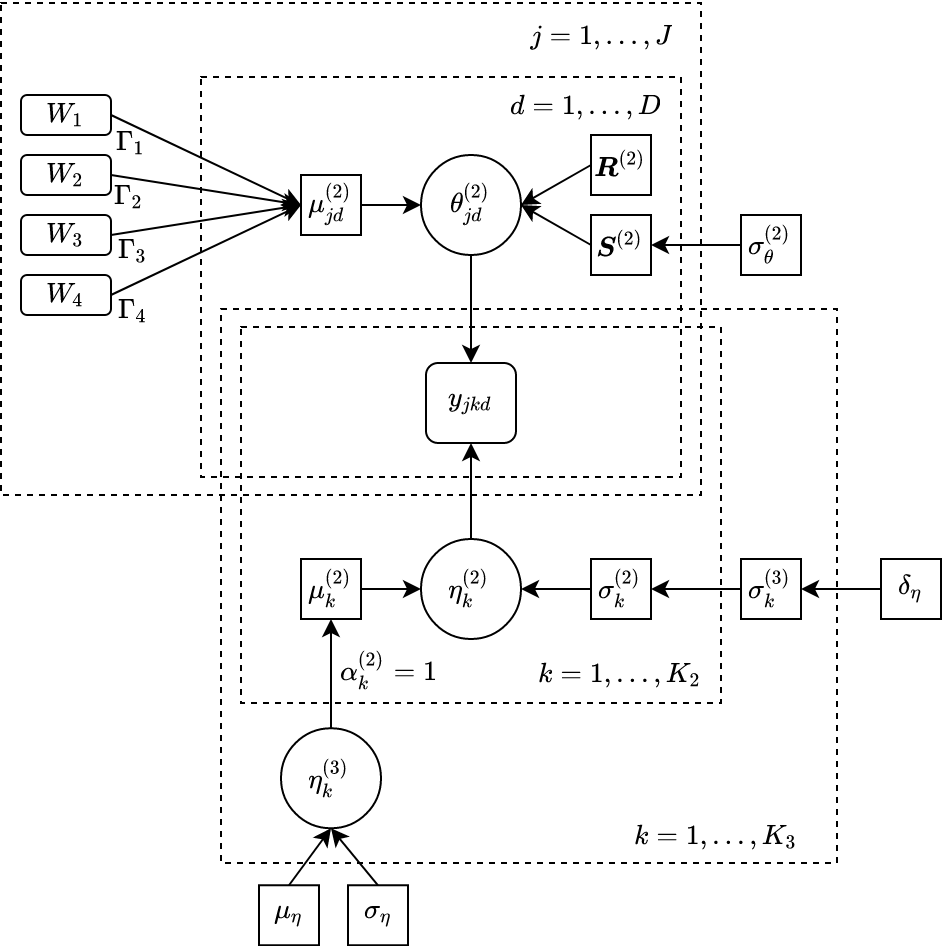
\includegraphics[width=0.7\linewidth]{4_FOLV_dag}
	%
	\caption[Directed Acyclig Graph (DAG). First Order Latent Variables model (FOLV).]%
	{Directed Acyclig Graph (DAG). First Order Latent Variables model (FOLV). Circles represent latent variables. Squares represent parameters or parameters for priors. Large Squares represent nesting in specific units.}
	\label{fig:FOLV_model}
\end{figure}
%
\begin{figure}[h]
	\centering
	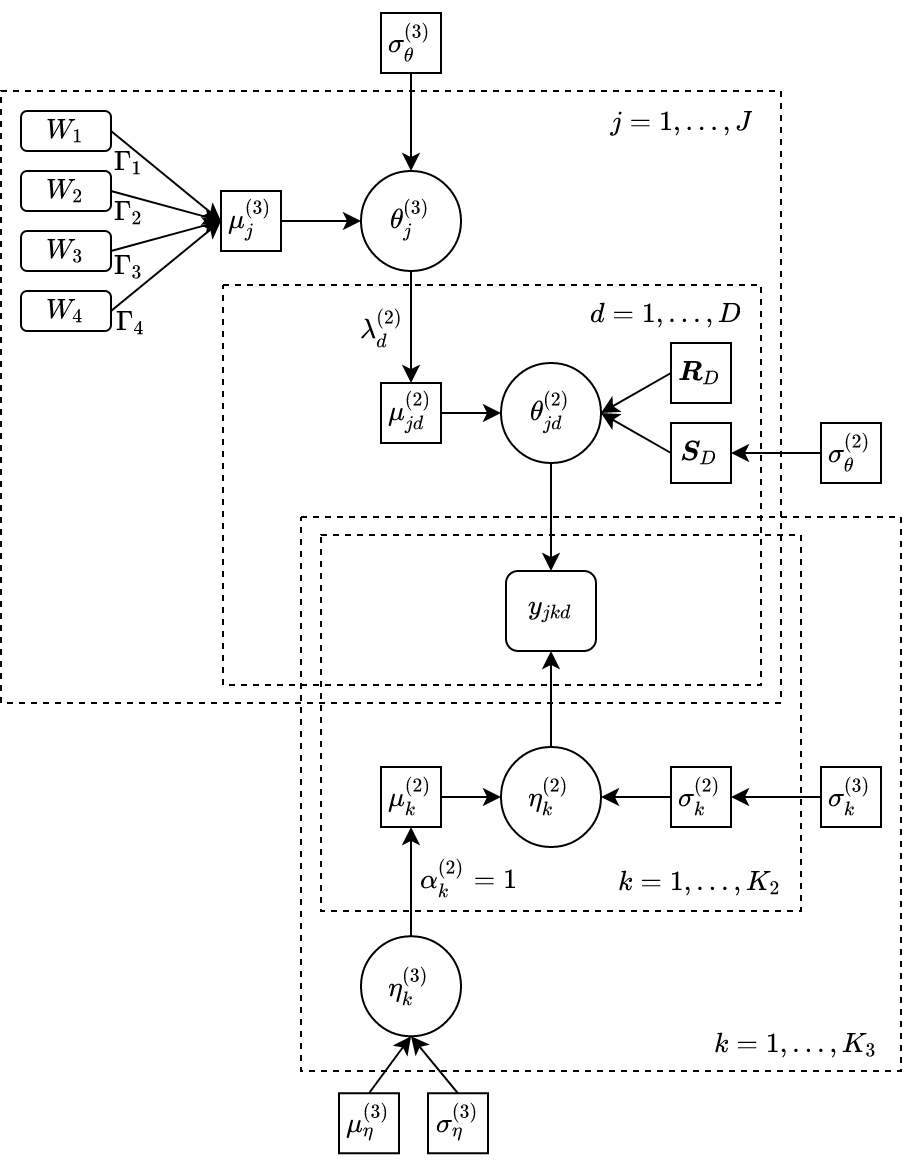
\includegraphics[width=0.7\linewidth]{4_SOLV_dag}
	%
	\caption[Directed Acyclic Graph (DAG). Second Order Latent Variables model (SOLV).]%
	{Directed Acyclig Graph (DAG). Second Order Latent Variables model (SOLV). Circles represent latent variables. Squares represent parameters or parameters for priors. Large Squares represent nesting in specific units.}
	\label{fig:SOLV_model}
\end{figure}

\subsection{FOLV CP}

\subsection{FOLV NCP}

\subsection{SOLV CP}

\subsection{SOLV NCP}

